\subsection{Representing and visualizing spatial transcriptomics experiments}\label{representing-and-visualizing-spatial-transcriptomics-experiments}}

Spatial transcriptomics (ST) allows the quantification of RNA expression of large numbers of genes while preserving the spatial context of tissues and cells. This is important as cancer progression depends on a complex tumor microenvironment, and not just cell type composition, but also cell type spatial organization can be used to derive diagnostic or prognostic markers.

The Bioconductor project offers multiple approaches to handle and manipulate
spatial transcriptomics data.
The SpatialExperiment class \cite{rig22} %(Righelli et al. \protect\hyperlink{ref-rig22}{2022}) 
is designed to be a lightweight,
technology-agnostic container. By inheriting from the
SingleCellExperiment class, it unlocks the use in ST data of
analysis packages designed for single-cell data, such as scater for exploration
and QC, and scran for normalization.
SpatialFeatureExperiment \cite{moses23} %(Moses et al. \protect\hyperlink{ref-moses23}{2023}) 
extends SpatialExperiment to easily
reuse polygons and other spatial geometry features from geospatial CRAN
packages, such as sf. See also MoleculeExperiment \cite{Couto2023} %(Couto et al. \protect\hyperlink{ref-Couto2023}{2023}) 
for a different
approach based on the data.table package.

In addition to data containers, Bioconductor provides a rich set of ST data.
The STexampleData and SFEData packages contain a collection of datasets from
different technologies and tissues.
As of December 2023,
the TENxVisiumData package provides a collection of 13 in-house 10X Genomics
Visium datasets from 23 samples across two organisms (human and mouse) and 13
tissues.
The MerfishData package contains two annotated samples assayed with the MERFISH
in-situ imaging protocol.

Finally, Bioconductor offers a growing collection of analysis methods tailored
for spot-based and in-situ ST data, including methods for visualization,
data exploration and quality control, spot deconvolution,
spatially-aware clustering, and identification of spatially-variable genes.

To show a simple example of an analysis workflow on spot-based data,
we explore a fresh frozen
Invasive Ductal Carcinoma breast tissue assayed
with the 10X Genomics Visium platform.
First, we use the ggspavis package for visualization.
See Figure \ref{fig:tenxvisium}.

%\begin{Shaded}
%\begin{Highlighting}[]
%\KeywordTok{library}\NormalTok{(TENxVisiumData)}
%\CommentTok{\#\# snapshotDate(): 2023{-}10{-}24}
%\KeywordTok{library}\NormalTok{(SpatialExperiment)}
%\CommentTok{\#\# 0/0 packages newly attached/loaded, see sessionInfo() for details.}
%\KeywordTok{library}\NormalTok{(ggspavis)}
%\CommentTok{\#\# 1/1 packages newly attached/loaded, see sessionInfo() for details.}
%\NormalTok{hbc \textless{}{-}}\StringTok{ }\KeywordTok{HumanBreastCancerIDC}\NormalTok{()}
%\CommentTok{\#\# see ?TENxVisiumData and browseVignettes(\textquotesingle{}TENxVisiumData\textquotesingle{}) for documentation}
%\CommentTok{\#\# loading from cache}
%\NormalTok{hbc \textless{}{-}}\StringTok{ }\NormalTok{hbc[,hbc}\OperatorTok{$}\NormalTok{sample\_id}\OperatorTok{==}\StringTok{"HumanBreastCancerIDC1"}\NormalTok{]}
%\NormalTok{hbc}\OperatorTok{$}\NormalTok{in\_tissue \textless{}{-}}\StringTok{ }\OtherTok{TRUE}
%\NormalTok{hbc \textless{}{-}}\StringTok{ }\KeywordTok{rotateImg}\NormalTok{(hbc, }\DataTypeTok{degrees=}\OperatorTok{{-}}\DecValTok{90}\NormalTok{)}
%\KeywordTok{plotVisium}\NormalTok{(hbc, }\DataTypeTok{y\_reverse =} \OtherTok{FALSE}\NormalTok{)}
%\end{Highlighting}
%\end{Shaded}

\begin{shaded}
\begin{verbatim}
library(TENxVisiumData)
## snapshotDate(): 2023-10-24
library(SpatialExperiment)
library(ggspavis)
hbc <- HumanBreastCancerIDC()
## see ?TENxVisiumData and browseVignettes('TENxVisiumData') for documentation
## loading from cache
hbc <- hbc[,hbc$sample_id=="HumanBreastCancerIDC1"]
hbc$in_tissue <- TRUE
hbc <- rotateImg(hbc, degrees=-90)
plotVisium(hbc, y_reverse = FALSE)
\end{verbatim}
\end{shaded}


\begin{figure}
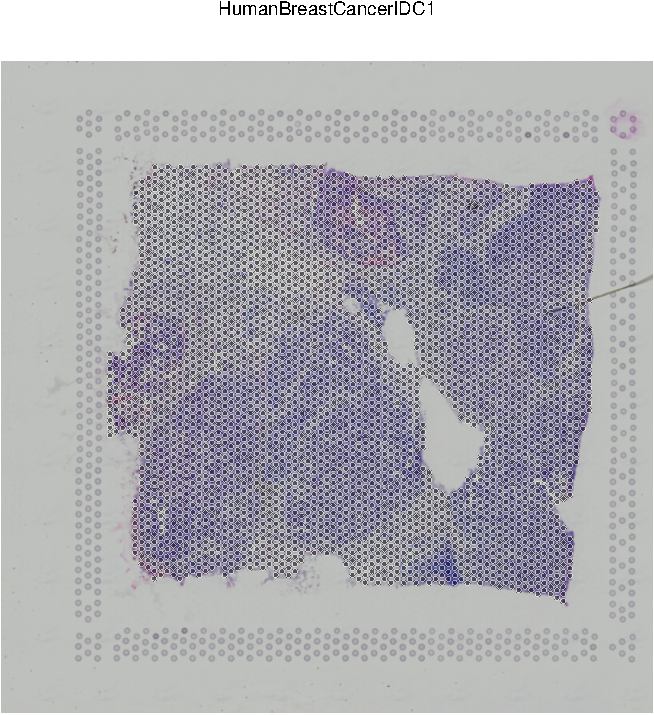
\includegraphics[width=1\linewidth,]{spatpdfs/tenxvisium-1} \caption{Visualization of a Visium breast cancer sample}\label{fig:tenxvisium}
\end{figure}

To investigate the spatially variable genes the nnSVG package
implements a method for the detection of genes whose expression varies in the
tissue spatial domains by fitting nearest-neighbor Gaussian processes 
\cite{webr23}.
%(Weber et al. \protect\hyperlink{ref-webr23}{2023}).

%\begin{Shaded}
%\begin{Highlighting}[]
%\KeywordTok{library}\NormalTok{(scater)}
%\CommentTok{\#\# 2/14 packages newly attached/loaded, see sessionInfo() for details.}
%\KeywordTok{library}\NormalTok{(nnSVG)}
%\CommentTok{\#\# 1/4 packages newly attached/loaded, see sessionInfo() for details.}
%\KeywordTok{library}\NormalTok{(scran)}
%\CommentTok{\#\# 1/9 packages newly attached/loaded, see sessionInfo() for details.}
%
%\CommentTok{\#add quality metrics}
%\NormalTok{is\_mito \textless{}{-}}\StringTok{ }\KeywordTok{grepl}\NormalTok{(}\StringTok{"(\^{}MT{-})|(\^{}mt{-})"}\NormalTok{, }\KeywordTok{rowData}\NormalTok{(hbc)}\OperatorTok{$}\NormalTok{symbol)}
%\NormalTok{hbc \textless{}{-}}\StringTok{ }\KeywordTok{addPerCellQC}\NormalTok{(hbc, }\DataTypeTok{subsets =} \KeywordTok{list}\NormalTok{(}\DataTypeTok{mito =}\NormalTok{ is\_mito))}
%
%\CommentTok{\#\# needed because the column name is hard coded in the nnSVG::filter\_genes}
%\KeywordTok{rowData}\NormalTok{(hbc)}\OperatorTok{$}\NormalTok{gene\_name \textless{}{-}}\StringTok{ }\KeywordTok{rowData}\NormalTok{(hbc)}\OperatorTok{$}\NormalTok{symbol }
%
%\CommentTok{\#\# filter and normalize gene expression}
%\NormalTok{hbc \textless{}{-}}\StringTok{ }\KeywordTok{filter\_genes}\NormalTok{(hbc)}
%\CommentTok{\#\# Gene filtering: removing mitochondrial genes}
%\CommentTok{\#\# removed 13 mitochondrial genes}
%\CommentTok{\#\# Gene filtering: retaining genes with at least 3 counts in at least 0.5\% (n = 19) of spatial locations}
%\CommentTok{\#\# removed 26583 out of 36588 genes due to low expression}
%\NormalTok{hbc \textless{}{-}}\StringTok{ }\KeywordTok{computeLibraryFactors}\NormalTok{(hbc)}
%\NormalTok{hbc \textless{}{-}}\StringTok{ }\KeywordTok{logNormCounts}\NormalTok{(hbc)}
%
%\CommentTok{\#\# select highly variable genes}
%\NormalTok{hvgs \textless{}{-}}\StringTok{ }\KeywordTok{getTopHVGs}\NormalTok{(hbc, }\DataTypeTok{n=}\DecValTok{1000}\NormalTok{)}
%\NormalTok{hbc \textless{}{-}}\StringTok{ }\NormalTok{hbc[hvgs,]}
%
%\CommentTok{\#\# identify spatially variable genes}
%\NormalTok{hbc \textless{}{-}}\StringTok{ }\KeywordTok{nnSVG}\NormalTok{(hbc, }\DataTypeTok{n\_threads=}\DecValTok{4}\NormalTok{)}
%
%\CommentTok{\#\# post{-}processing}
%\NormalTok{hbc \textless{}{-}}\StringTok{ }\NormalTok{hbc[}\KeywordTok{order}\NormalTok{(}\KeywordTok{rowData}\NormalTok{(hbc)}\OperatorTok{$}\NormalTok{rank),]}
%
%\NormalTok{gnr1 \textless{}{-}}\StringTok{ }\KeywordTok{rowData}\NormalTok{(hbc)}\OperatorTok{$}\NormalTok{symbol[}\DecValTok{1}\NormalTok{]}
%\KeywordTok{rownames}\NormalTok{(hbc) \textless{}{-}}\StringTok{ }\KeywordTok{rowData}\NormalTok{(hbc)}\OperatorTok{$}\NormalTok{symbol}
%\end{Highlighting}
%\end{Shaded}

\begin{shaded}
\begin{verbatim}
library(scater)
library(nnSVG)
library(scran)
#add quality metrics
is_mito <- grepl("(ˆMT-)|(ˆmt-)", rowData(hbc)$symbol)
hbc <- addPerCellQC(hbc, subsets = list(mito = is_mito))
## needed because the column name is hard coded in the nnSVG::filter_genes
rowData(hbc)$gene_name <- rowData(hbc)$symbol
## filter and normalize gene expression
hbc <- filter_genes(hbc)
## Gene filtering: removing mitochondrial genes
## removed 13 mitochondrial genes
## Gene filtering: retaining genes with at least 3 counts in at least 0.5% (n = 19) of spatial locations
## removed 26583 out of 36588 genes due to low expression
hbc <- computeLibraryFactors(hbc)
hbc <- logNormCounts(hbc)
## select highly variable genes
hvgs <- getTopHVGs(hbc, n=1000)
hbc <- hbc[hvgs,]
## identify spatially variable genes
hbc <- nnSVG(hbc, n_threads=4)
## post-processing
hbc <- hbc[order(rowData(hbc)$rank),]
gnr1 <- rowData(hbc)$symbol[1]
rownames(hbc) <- rowData(hbc)$symbol
\end{verbatim}
\end{shaded}

By ranking the results of nnSVG, we are able to detect the most spatially
variable genes. As an example, we show how the most spatially variable gene varies
across the tissue.

%\begin{Shaded}
%\begin{Highlighting}[]
%\KeywordTok{plotVisium}\NormalTok{(hbc, }\DataTypeTok{y\_reverse =} \OtherTok{FALSE}\NormalTok{, }\DataTypeTok{fill =}\NormalTok{ gnr1, }\DataTypeTok{palette=}\StringTok{"red"}\NormalTok{)}
%\end{Highlighting}
%\end{Shaded}

\begin{shaded}
\begin{verbatim}
plotVisium(hbc, y_reverse = FALSE, fill = gnr1, palette="red")
\end{verbatim}
\end{shaded}

\begin{figure}
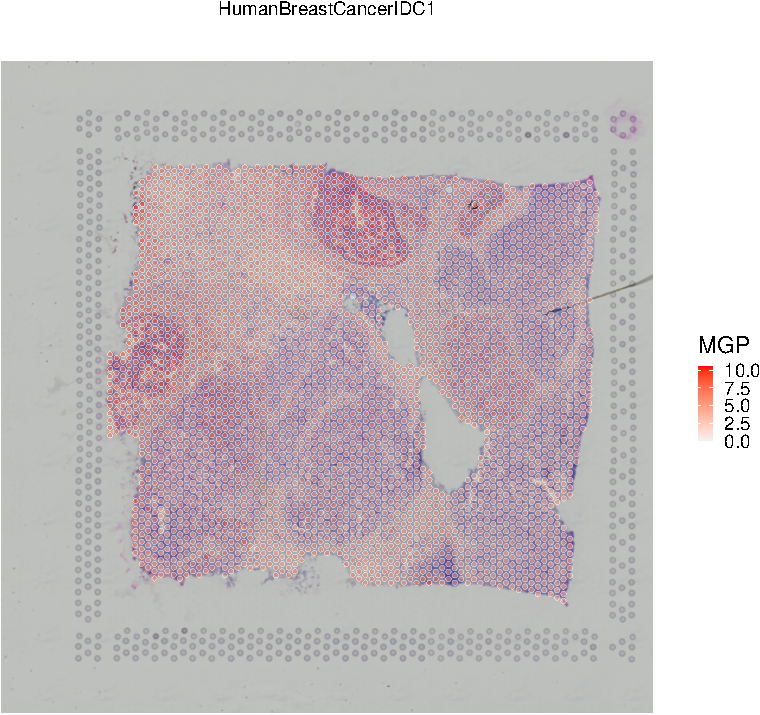
\includegraphics[width=1\linewidth,]{spatpdfs/plotvisium-1} \caption{Spatial expression of a highly variable gene}\label{fig:plotvisium}
\end{figure}

Finally, we show an example of an in-situ ST technology, by visualizing a breast
cancer sample assayed with the 10X Genomics Xenium platform.

\begin{shaded}
\begin{verbatim}
library(SpatialFeatureExperiment)
library(SFEData)
jbr = JanesickBreastData("rep1")
jbr
## class: SpatialFeatureExperiment
## dim: 541 167782
## metadata(1): Samples
## assays(1): counts
## rownames(541): ABCC11 ACTA2 ... BLANK_0497 BLANK_0499
## rowData names(6): ID Symbol ... vars cv2
## colnames: NULL
## colData names(10): Sample Barcode ... nCounts nGenes
## reducedDimNames(0):
## mainExpName: NULL
## altExpNames(0):
## spatialCoords names(2) : x_centroid y_centroid
## imgData names(1): sample_id
##
## unit:
## Geometries:
## colGeometries: centroids (POINT), cellSeg (POLYGON), nucSeg (GEOMETRY)
##
## Graphs:
## sample01:
\end{verbatim}
\end{shaded}

%\begin{Shaded}
%\begin{Highlighting}[]
%\KeywordTok{library}\NormalTok{(SpatialFeatureExperiment)}
%\KeywordTok{library}\NormalTok{(SFEData)}
%\NormalTok{jbr =}\StringTok{ }\KeywordTok{JanesickBreastData}\NormalTok{(}\StringTok{"rep1"}\NormalTok{)}
%\NormalTok{jbr}
%\CommentTok{\#\# class: SpatialFeatureExperiment }
%\CommentTok{\#\# dim: 541 167782 }
%\CommentTok{\#\# metadata(1): Samples}
%\CommentTok{\#\# assays(1): counts}
%\CommentTok{\#\# rownames(541): ABCC11 ACTA2 ... BLANK\_0497 BLANK\_0499}
%\CommentTok{\#\# rowData names(6): ID Symbol ... vars cv2}
%\CommentTok{\#\# colnames: NULL}
%\CommentTok{\#\# colData names(10): Sample Barcode ... nCounts nGenes}
%\CommentTok{\#\# reducedDimNames(0):}
%\CommentTok{\#\# mainExpName: NULL}
%\CommentTok{\#\# altExpNames(0):}
%\CommentTok{\#\# spatialCoords names(2) : x\_centroid y\_centroid}
%\CommentTok{\#\# imgData names(1): sample\_id}
%\CommentTok{\#\# }
%\CommentTok{\#\# unit:}
%\CommentTok{\#\# Geometries:}
%\CommentTok{\#\# colGeometries: centroids (POINT), cellSeg (POLYGON), nucSeg (GEOMETRY) }
%\CommentTok{\#\# }
%\CommentTok{\#\# Graphs:}
%\CommentTok{\#\# sample01:}
%\end{Highlighting}
%\end{Shaded}

We can leverage the nature of in-situ data to explore the cell density across the
tissue, identifying the tissue's macrostructure, and the cell segmentation,
zooming in on a small portion of the tissue.

\begin{shaded}
\begin{verbatim}
library(Voyager)
cellbins <- plotCellBin2D(jbr, hex = TRUE)
cellgeo <- plotGeometry(jbr, "cellSeg", bbox=c("xmin"=0, "ymin"=4000, "xmax"=1000, "ymax"=5000))
library(gridExtra)
grid.arrange(cellbins, cellgeo, ncol=2)
\end{verbatim}
\end{shaded}

\begin{figure}
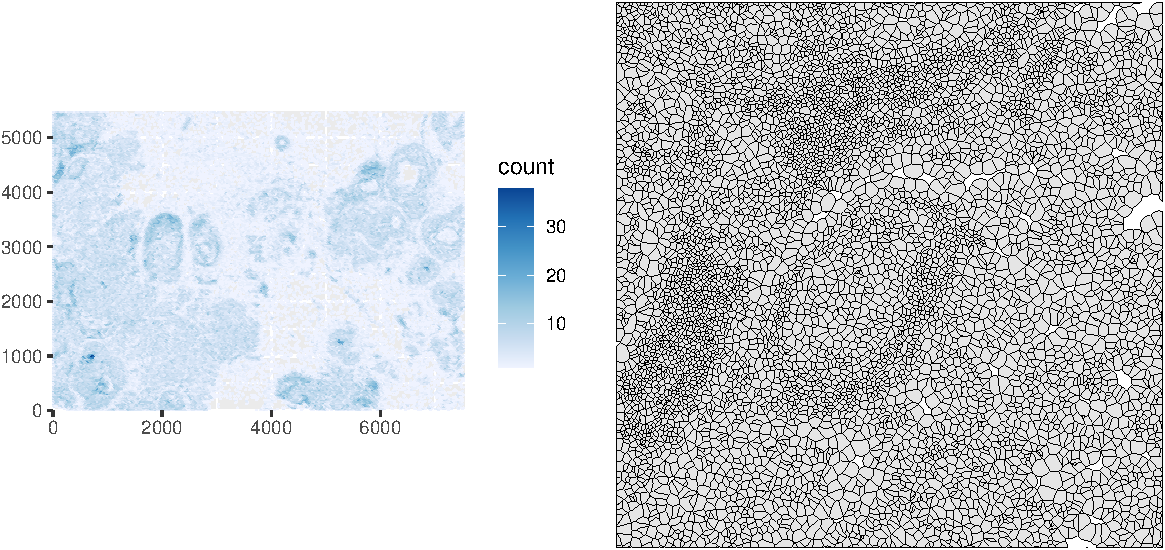
\includegraphics[width=1\linewidth,]{spatpdfs/plotvoyager-1} \caption{Cell density and cell boundaries of a Xenium breast cancer sample}\label{fig:plotvoyager}
\end{figure}

Finally, we can visualize the expression of marker genes after log-normalizing
the data.

\begin{shaded}
\begin{verbatim}
jbr <- jbr[, jbr$nCounts >= 20]
jbr <- logNormCounts(jbr)
library(scattermore)
## 1/0 packages newly attached/loaded, see sessionInfo() for details.
strom <- plotSpatialFeature(jbr, "POSTN", colGeometryName = "centroids",
scattermore = TRUE, ncol = 2, pointsize = 0.5) + ggtitle("POSTN, stromal")
fasn <- plotSpatialFeature(jbr, "FASN", colGeometryName = "centroids",
scattermore = TRUE, ncol = 2, pointsize = 0.5) +
ggtitle("FASN, invasive")
grid.arrange(strom, fasn, ncol=2)
\end{verbatim}
\end{shaded}

%\begin{Shaded}
%\begin{Highlighting}[]
%\NormalTok{jbr \textless{}{-}}\StringTok{ }\NormalTok{jbr[, jbr}\OperatorTok{$}\NormalTok{nCounts }\OperatorTok{\textgreater{}=}\StringTok{ }\DecValTok{20}\NormalTok{]}
%\NormalTok{jbr \textless{}{-}}\StringTok{ }\KeywordTok{logNormCounts}\NormalTok{(jbr)}
%\KeywordTok{library}\NormalTok{(scattermore)}
%\CommentTok{\#\# 1/0 packages newly attached/loaded, see sessionInfo() for details.}
%\NormalTok{strom \textless{}{-}}\StringTok{ }\KeywordTok{plotSpatialFeature}\NormalTok{(jbr, }\StringTok{"POSTN"}\NormalTok{, }\DataTypeTok{colGeometryName =} \StringTok{"centroids"}\NormalTok{,}
%                   \DataTypeTok{scattermore =} \OtherTok{TRUE}\NormalTok{, }\DataTypeTok{ncol =} \DecValTok{2}\NormalTok{, }\DataTypeTok{pointsize =} \FloatTok{0.5}\NormalTok{) }\OperatorTok{+}
%\StringTok{  }\KeywordTok{ggtitle}\NormalTok{(}\StringTok{"POSTN, stromal"}\NormalTok{)}
%
%\NormalTok{fasn \textless{}{-}}\StringTok{ }\KeywordTok{plotSpatialFeature}\NormalTok{(jbr, }\StringTok{"FASN"}\NormalTok{, }\DataTypeTok{colGeometryName =} \StringTok{"centroids"}\NormalTok{,}
%                   \DataTypeTok{scattermore =} \OtherTok{TRUE}\NormalTok{, }\DataTypeTok{ncol =} \DecValTok{2}\NormalTok{, }\DataTypeTok{pointsize =} \FloatTok{0.5}\NormalTok{) }\OperatorTok{+}
%\StringTok{  }\KeywordTok{ggtitle}\NormalTok{(}\StringTok{"FASN, invasive"}\NormalTok{)}
%
%\KeywordTok{grid.arrange}\NormalTok{(strom, fasn, }\DataTypeTok{ncol=}\DecValTok{2}\NormalTok{)}
%\end{Highlighting}
%\end{Shaded}

\begin{figure}
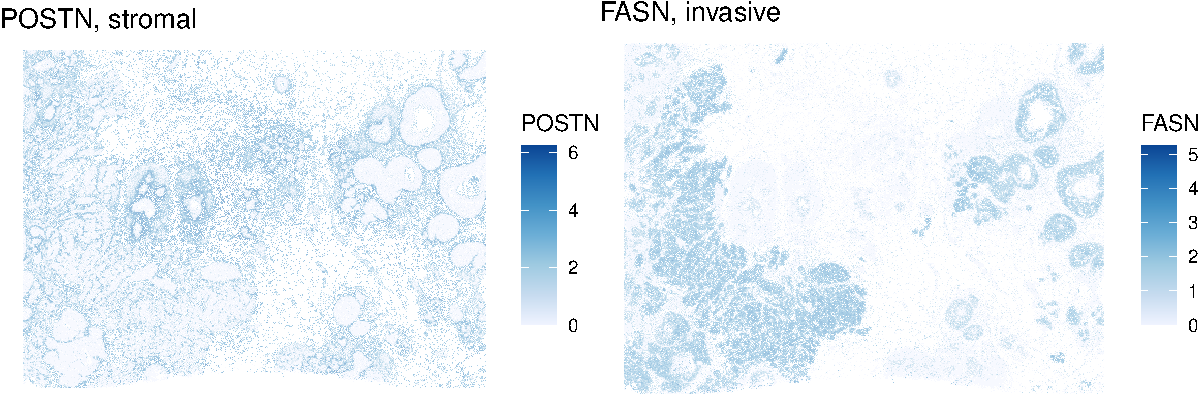
\includegraphics[width=1\linewidth,]{spatpdfs/sfemark-1} \caption{Spatial expression of marker genes}\label{fig:sfemark}
\end{figure}

